\section{Репликация Tarantool}

В данном разделе будет подробно рассмотрен механизм репликации в СУБД Tarantool. Будет описано, как Tarantool обеспечивает передачу данных между узлами в репликасете, чтобы поддерживать актуальность и согласованность данных на всех репликах. Также будет рассмотрено, как осуществляется настройка репликасетов, выбор ведущего узла и подключение анонимных реплик. Особое внимание будет уделено протоколу подключения новых реплик в уже существующий репликасет.


\subsection{Общая информация}

В Tarantool группа узлов, которые работают с копиями одной и той же базы данных, объединяется в репликасет. Внутри репликасета каждому узлу назначается определенная роль: мастер или реплика. Только мастер может обрабатывать DDL, DML и DCL запросы, реплики же обрабатывают только DQL.

Репликация представляет собой процесс копирования данных с одного узла на другие узлы в репликасете. В Tarantool репликация происходит не только с мастеров на реплики, но и с реплик на реплики. Репликация в базе данных необходима для решения следующих проблем:

\begin{enumerate}
    \item Обеспечение отказоустойчивости. Репликация позволяет создать несколько копий данных на разных узлах или серверах. В случае сбоя одного из узлов (например, из-за аппаратных проблем или аварийного отключения), другие узлы, содержащие реплики данных, могут продолжить обслуживание запросов, минимизируя простой системы и предотвращая потерю данных;
    \item Масштабирование чтения. За счет репликации можно распределять нагрузку на чтение между несколькими узлами. Это особенно полезно в системах, где количество операций чтения значительно превышает количество операций записи. Реплики могут обрабатывать запросы на чтение, разгружая ведущий узел, что улучшает общую производительность сервиса.
    \item Географическое распределение данных. В распределенных системах, где пользователи могут находиться в разных географических регионах, репликация позволяет разместить копии данных ближе к конечным пользователям. Это снижает задержки при доступе к данным и улучшает пользовательский опыт.
\end{enumerate}

Реплика непрерывно получает обновления данных от мастера или от другой реплики, применяя журнал записей операций WAL. Каждая запись в журнале представляет собой отдельный запрос (DDL, DML, DCL) и имеет монотонно растущий номер (LSN). WAL журналы в Tarantool представлены xlog файлами. Tarantool хранит snapshot файл, который содержит полное состояние БД в конкретный момент времени, и xlog файлы с момента записи последнего снапшота. Репликация ведется только из xlog файлов.

Tarantool поддерживает два типа репликации:

\begin{enumerate}
    \item Синхронная репликация. Обеспечивает высокую степень консистентности данных, так как изменения записываются на мастере и подтверждаются всеми репликами, участвующими в кворуме, прежде чем клиент получает подтверждение выполнения операции. Этот тип репликации минимизирует риск потери данных, но может увеличивать задержки при записи из-за необходимости ожидания подтверждения от всех реплик.
    \item Асинхронная репликация. Изменения данных сначала записываются на мастере, а затем передаются на реплики без ожидания их подтверждения. Это позволяет снизить задержки при записи, но может привести к временной неконсистентности данных на разных узлах и потенциальной потере данных в случае сбоя мастера.
\end{enumerate}

Так как CDC не заинтересован в сихронной репликации, мы не будем рассмотривать ее подробно.


\subsection{Настройка репликасета}

\textbf{Шаг 1. Подготовка узлов}

Для настройки репликасета необходимо подготовить несколько узлов, на которых будет запущен Tarantool. Каждый узел должен быть настроен и доступен для связи с другими узлами в кластере. Необходимо убедиться, что на каждом узле установлена одна и та же версия Tarantool. В примере настройка репликасета производится локально, на одном компьютере. \\

\textbf{Шаг 2. Конфигурация мастера}

Первым шагом является настройка мастера, который будет основным источником данных для репликации. Его необходимо сконфигурировать со следующими параметрами \cite{TarantoolDoc}:

\begin{itemize}
    \item \textit{listen} - URI, на котором узел принимает входящие подключения.
    \item \textit{replication} - список URI, с которых узел реплицирует данные.
\end{itemize}

Пример конфигурирования мастера приведен на рисунке~\ref{fig:fig01}.

\begin{figure}
  \centering
  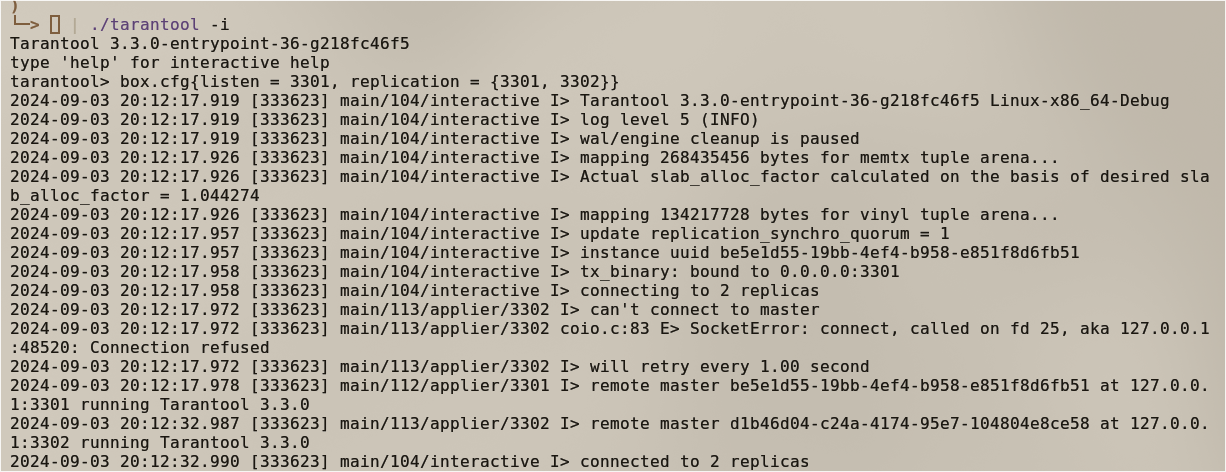
\includegraphics[scale=0.35]{inc/master.png}
  \caption{Конфигурация мастера}
  \label{fig:fig01}
\end{figure}

\textbf{Шаг 3. Конфигурация реплики}

Реплики настраиваются аналогичным образом, но с указанием опции \textit{read\_only}, устанавливающей режим только для чтения, чтобы запретить выполнение операций записи на реплике. Реплику можно сделать анонимной, указав параметр \textit{replication\_anon}.

\textbf{Шаг 4. Проверка состояния репликасета}

После настройки и запуска всех узлов необходимо убедиться, что репликасет работает корректно. Сделать это можно с помощью \textit{box.info.replication}, как показано на рисунке~\ref{fig:fig03}. Эта команда включает информацию о подключении к узлу, статусе синхронизации (\textit{vclock}) и задержке (\textit{lag}) \cite{TarantoolDoc}.

\begin{figure}
  \centering
  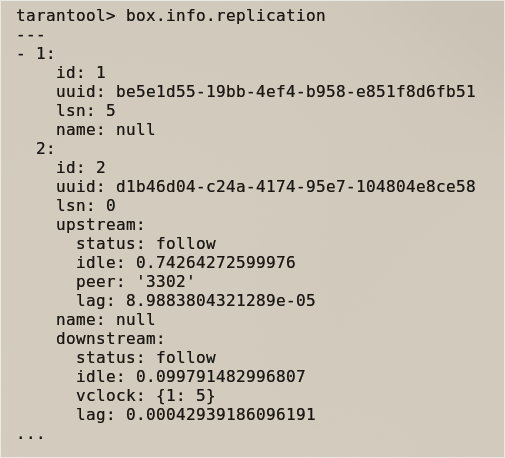
\includegraphics[scale=0.35]{inc/master-info.png}
  \caption{Состояние подключения узла}
  \label{fig:fig03}
\end{figure}


\subsection{Подключение узла к репликасету}

В данной части описывается протокол подключения реплики, так как это необходимо для понимания решений, предлагаемых к поставленным во введении задачам.

\begin{enumerate}
    \item В ходе конфигурации реплика генерирует UUID, являющийся уникальным идентификатором этого узла в репликасете. Для каждого URI в \textit{box.cfg.replication} создается сущность, называемая applier, задача которой состоит в применении данных, получаемых от мастера. Applier инициирует подключение к мастеру.
    \item Applier посылает сообщение IPROTO\_JOIN, при получении которого мастер создает relay, нужный для пересылки изменений БД на реплику. IPROTO\_JOIN представляет собой запрос на добавление узла к кластеру и необходим для получение начального состояния с мастера. Процесс отсылки начального состояния делится на две фазы.
    \item Initial JOIN. Мастер создает read-view (снимок) текущего состояние БД и посылает его реплике. По окончании initial JOIN мастер добавляет узел в репликасет путем вставки UUID реплики с соответсвующим ID в спейс \_cluster.
    \item Final JOIN. С момента создания read-view до окончания его пересылки может пройти много времени и состоянии БД наверняка изменится. Потому в фазе final JOIN мастер посылает все изменения, появившиеся со времени начала пересылки read-view.
    \item По окончании JOIN, реплика посылает запрос IPROTO\_SUBSCRIBE. Мастер отвечает своим текущим vclock-ом. С этого момента реплика переходит в стадию FOLLOW, она применяет все обновления WAL, исходящие от мастера.
\end{enumerate}

В Tarantool также есть возможность создания анонимных реплик, которые не являются участником репликасета, не могут становиться мастером, не учавствуют в кворуме синхронной репликации. Однако они получают и применяют поток репликационных данных. Вместо IPROTO\_JOIN они посылают IPROTO\_FETCH\_SNAPSHOT, который выполняет только первую фазу подключения: initial JOIN. Анонимные реплики не добавляются в спейс \_cluster. В любой момент анонимная реплика может стать обычной, послав запрос IPROTO\_REGISTER.
